% Packages
% sudo tlmgr install silence appendixnumberbeamer fira fontaxes mwe noto csquotes babel helvet
%--- Preamble ---------------------------------------------------------%
% Load LaTeX packages
\documentclass[aspectratio=169]{beamer}                    % supports floating text in any location
\usetheme[darkmode]{pureminimalistic}
%\usetheme[lightmode]{pureminimalistic}
\graphicspath{
    {logos/}
    {../figures/}
    {images}
    }

\usepackage[utf8]{inputenc}
\usepackage{csquotes,xpatch}% recommended
%\usepackage[english]{babel}
%\usepackage[american]{babel}
\usepackage[brazil]{babel}
\babelprovide[import, main]{portuguese}
\babelprovide[import]{english}

\usepackage{tikz}
\usetikzlibrary{shapes}
\usetikzlibrary{arrows}
\usetikzlibrary{positioning}
\usetikzlibrary{calc}
\usetikzlibrary{fit}

% Desenho da Rede Neural
% Adaptado de https://latexdraw.com/drawing-neural-networks-in-tikz-short-guide/
% Input layer neurons' number
\newcommand{\inputnum}{2}
% Hidden layer neurons' number
\newcommand{\hiddennum}{3}
% Output layer neurons' number
\newcommand{\outputnum}{1}
\tikzset{
    pics/neuralnetwork/.style n args={3}{
        code= {
            % Input Layer
            \foreach \i in {1,...,#1}
            {
                \node[circle,
                    minimum size = 6mm,
                    fill=orange!30] (Input-\i) at (0,-\i) {};
            }
            % Hidden Layer
            \foreach \i in {1,...,#2}
            {
                \node[circle,
                    minimum size = 6mm,
                    fill=teal!50,
                    yshift=(#2-#1)*5 mm
                ] (Hidden-\i) at (2.5,-\i) {};
            }
            % Output Layer
            \foreach \i in {1,...,#3}
            {
                \node[circle,
                    minimum size = 6mm,
                    fill=purple!50,
                    yshift=(#3-#1)*5 mm
                ] (Output-\i) at (5,-\i) {};
            }
            % Connect neurons In-Hidden
            \foreach \i in {1,...,#1}
            {
                \foreach \j in {1,...,#2}
                {
                    \draw[->, shorten >=1pt, draw=white] (Input-\i) -- (Hidden-\j);
                }
            }
            % Connect neurons Hidden-Out
            \foreach \i in {1,...,#2}
            {
                \foreach \j in {1,...,#3}
                {
                    \draw[->, shorten >=1pt, draw=white] (Hidden-\i) -- (Output-\j);
                }
            }
        }
    }
    neuralnetwork/.style={node contents=\usebox{\Chart}}
}

\newsavebox\Chart
\sbox\Chart{
    \begin{tikzpicture}[auto,>=latex']
        % Input Layer
        \foreach \i in {1,...,3}
        {
            \node[circle,
                minimum size = 6mm,
                fill=orange!30] (Input-\i) at (0,-\i) {};
        }
        % Hidden Layer
        \foreach \i in {1,...,2}
        {
            \node[circle,
                minimum size = 6mm,
                fill=teal!50,
                yshift=(2-3)*5 mm
            ] (Hidden-\i) at (1.25,-\i) {};
        }
        % Output Layer
        \foreach \i in {1,...,1}
        {
            \node[circle,
                minimum size = 6mm,
                fill=purple!50,
                yshift=(1-3)*5 mm
            ] (Output-\i) at (2.5,-\i) {};
        }
        % Connect neurons In-Hidden
        \foreach \i in {1,...,3}
        {
            \foreach \j in {1,...,2}
            {
                \draw[->, shorten >=1pt, draw=white] (Input-\i) -- (Hidden-\j);
            }
        }
        % Connect neurons Hidden-Out
        \foreach \i in {1,...,2}
        {
            \foreach \j in {1,...,1}
            {
                \draw[->, shorten >=1pt, draw=white] (Hidden-\i) -- (Output-\j);
            }
        }
    \end{tikzpicture}}

\usepackage{pgfplots}
\pgfplotsset{height=7cm,  % only if needed
             width=12cm,  % only if needed
             compat=1.17, % only if needed
             legend style = {fill = black, draw = white}}

\usepackage{tabularx}
\usepackage{booktabs}
\usepackage{hyperref}
\usepackage{float}

% \renewcommand{\pageword}{}
% \renewcommand{\logoheader}{\vspace{1.5em}}

\usepackage[
%    natbib=true,
    backend=biber,
%    style=abnt,
%    style=authoryear-comp,
%    style=authoryear,
%    style=ieee,
%    style=acm,
    style=apa,
%    style=siam,
%    style=ieeetr,
%    style=plain,
    doi=true,
    eprint=false,
    hyperref=true]
    {biblatex}
\addbibresource{references.bib}

%% this makes it possible to add backup slides, without counting them
\usepackage{appendixnumberbeamer}
\renewcommand{\appendixname}{\texorpdfstring{\translate{appendix}}{appendix}}

% logos

% footer page
\renewcommand{\pageword}{Página}

% Math Font Default (Fira is strange)
\renewcommand\mathfamilydefault{\rmdefault}

% if loaded after begin{document} a warning will appear: "pdfauthor already used"
\title[COVID-19, Epidemiologia e Redes Sociais]{COVID-19, Epidemiologia e Redes Sociais}
\author{Jose Storopoli, Alessandra Pellini e André Santos \\
\texttt{josees@uni9.pro.br}}
\institute{Universidade Nove de Julho - UNINOVE}
\date{\today}

\begin{document}
% has to be loaded outside of a frame to work!
\maketitle

% For longer table of contents, I find it cleaner to
% use no footline.
\begin{frame}[plain, noframenumbering]{Outline}
    \tableofcontents
\end{frame}

\begin{frame}[plain, noframenumbering]{Licença}
    \begin{columns}
        \begin{column}{0.5\textwidth}
            O texto e as figuras desses slides possuem uma
            \href{https://creativecommons.org/licenses/by-nc-sa/4.0/deed.pt}{Licença
            Creative Commons
            Atribuição-NãoComercial-CompartilhaIgual 4.0 Internacional (CC BY-NC-SA 4.0)}
            \vfill
            \centering
            
\includegraphics[width=0.6\columnwidth]{CC_NC_SA.png}
        \end{column}
        \begin{column}{0.5\textwidth}
            \centering
            
\includegraphics[width=0.8\columnwidth]{QR_Code.png}
        \end{column}
    \end{columns}
    \vfill
\end{frame}

\section{LabCidades UNINOVE}
\begin{frame}{LabCidades UNINOVE}
    \begin{columns}
        \begin{column}{0.8\textwidth}
            \begin{vfilleditems}
                \item O Laboratório de Políticas Públicas e Cidades Inteligentes da UNINOVE possui como objetivo elaborar pesquisas para apoio à:
                \begin{vfilleditems}
                    \small
                    \item formulação de políticas públicas
                    \item tomada de decisão
                \end{vfilleditems}
                \item As principais técnicas são:
                \begin{vfilleditems}
                    \small
                    \item modelos \textcolor{blue}{estatísticos Bayesianos}
                    \item algoritmos de \textcolor{blue}{aprendizagem de máquina}
                    \item sistemas baseados em \textcolor{red}{evidências}
                \end{vfilleditems}
                \item Contexto de atuação:
                \begin{vfilleditems}
                    \small
                    \item Big Data
                    \item ferramentas \textit{open source}
                    \item \textit{Open science}: \footnotesize dados e código abertos para \textbf{replicabilidade} e \textbf{transparência}
                \end{vfilleditems}
            \end{vfilleditems}
        \end{column}
        \begin{column}{0.2\textwidth}
            \centering
            Placeholder Logo LabCidades
        \end{column}
    \end{columns}
    \centering
    Slides, códigos e dados disponíveis em \href{https://github.com/LabCidades/COVID-Classifier}{\texttt{LabCidades/COVID-Classifier}}
\end{frame}

\begin{frame}{LabCidades UNINOVE - Equipe}
    \begin{vfilleditems}
        \item Pesquisador Responsável: \href{https://github.com/storopoli}{Jose Storopoli}
        \item Pesquisador Associado: \href{https://github.com/acgpellini}{Alessandra Pellini}
        \item Pesquisador Assistente: \href{https://github.com/andrelmfsantos}{André Santos}
        \item Pesquisador Assistente: Lorenzo Gottardi
        \item Alunos de Iniciação Científica:
        \begin{vfilleditems}
            \item \href{https://github.com/vinivieiran}{João Vinícius Vieira Nóia}
            \item \href{https://github.com/Elias-Noda}{Elias Noda}
            \item \href{https://github.com/Paula-Fraga}{Paula Fraga}
            \item \href{https://github.com/camibrichta}{Camila Brichta}
            \item \href{https://github.com/leandrors91}{Leandro dos Santos}
            \item \href{https://github.com/juniorghostinthewires}{Junior De Sousa Silva}
        \end{vfilleditems}
    \end{vfilleditems}
    Slides, códigos e dados disponíveis em \href{https://github.com/LabCidades/COVID-Classifier}{\texttt{LabCidades/COVID-Classifier}}
\end{frame}

\section{Por que é dificil modelar e prever COVID-19?}
\begin{frame}{Por que é dificil modelar e prever COVID-19?}
    \begin{columns}
        \begin{column}{0.3\textwidth}
            Primeiramente porque estamos fazendo errado \parencite{ioannidisForecastingCOVID19Has2020}
        \end{column}
        \begin{column}{0.7\textwidth}
            \begin{vfilleditems}
                \item input pobres de dados
                \item suposições incorretas de modelagem
                \item alta instabilidade de estimativas
                \item falta de incorporação de características epidemiológicas
                \item falta de transparência
                \item consideração de apenas uma ou algumas dimensões do problema em questão
                \item falta de \textit{expertise}
                \item \textit{groupthink} e efeitos \textit{bandwagon}
                \item \textit{selective reporting}
            \end{vfilleditems}
        \end{column}
    \end{columns}
\end{frame}

\begin{frame}{Por que é dificil modelar e prever COVID-19?}
    \begin{columns}
        \begin{column}{0.4\textwidth}
            Mas alguns (não todos) desses problemas podem ser corrigidos \parencite{ioannidisForecastingCOVID19Has2020}
        \end{column}
        \begin{column}{0.6\textwidth}
            \begin{vfilleditems}
                \item Modelagem consciente de \textbf{distribuições preditivas} em vez de focar em estimativas pontuais
                \item considerando \textbf{dimensões múltiplas de impacto}
                \item reavaliando continuamente os modelos com base em seu \textbf{desempenho validado}
            \end{vfilleditems}
        \end{column}
    \end{columns}
\end{frame}

\begin{frame}{o Problema do $R_t$}
    A fórmula do $R_t$ (número efetivo de reprodução) é:
    $$R_t = R_0 \cdot \frac{S}{N}$$
    \vfill
    onde $R_0$ é o número básico de reprodução e $\frac{S}{N}$ é a proporção de suscetíveis $S$ da população $N$.
    \vfill
    Mas não sabemos os suscetíveis porque não temos testagem aleatórias para saber quantos $N$ estão infectados e além disso aproximações de $I$ por sintomas é complicado por conta da alta taxa de $I$ assintomáticos \parencite{gaoSystematicReviewAsymptomatic2021}:
    \begin{vfilleditems}
        \item 30.8\% - China, Wuhan \parencite{nishiura2020estimation}
        \item 51.7\% Navio Diamond Princess \parencite{mizumoto2020estimating}
    \end{vfilleditems}
\end{frame}

\section{Modelos Epidemiológicos Bayesianos}
\begin{frame}{Modelos SIR}
    \begin{columns}
        \begin{column}{0.5\textwidth}
            \begin{vfilleditems}
                \item Modelos compartimentais são usados para modelar a dinâmica de uma doença infecciosa em uma escala populacional
                \item Originados no início do século 20 com o modelo \textit{Susceptible-Infectious-Recovered} (SIR) \parencite{kermack1927contribution}
            \end{vfilleditems}
        \end{column}
        \begin{column}{0.5\textwidth}
            \begin{figure}
                \centering
                \begin{tikzpicture}[node distance=0.75cm,auto,>=latex',every node/.append style={align=center},int/.style={draw, circle, minimum size=0.9cm}]
                    \node [int] (S) {$S$};
                    \node [int, right=of S] (I) {$I$};
                    \node [int, right=of I] (R) {$R$};

                    \path[->, auto=false] (S) edge node {$\beta S \frac{I}{N}$ \\[2.5em]} (I);
                    \path[->, auto=false] (I) edge node {$\gamma I$ \\[2.5em]} (R);
                \end{tikzpicture}
                \label{fig:SIR}
                \caption{Modelo SIR}
            \end{figure}
        \end{column}
    \end{columns}
\end{frame}

\begin{frame}{Modelo SIRTD}
    \begin{columns}
        \begin{column}{0.5\textwidth}
            \begin{vfilleditems}
                \item Algumas doenças infecciosas são fatais, portanto, para diferenciar entre os recuperados e os mortos, foi desenvolvido o modelo (SIRD) \parencite{bailey1975mathematical}
                \item Como a COVID-19 pode superar rapidamente o sistema de saúde de uma nação \parencite{pintonetoMathematicalModelCOVID192021}, há a necessidade de incluir um estado que represente pacientes terminais $T$ (SIRTD).
            \end{vfilleditems}
        \end{column}
        \begin{column}{0.5\textwidth}
            \begin{figure}
                \centering
                \begin{tikzpicture}[node distance=0.75cm,auto,>=latex',every node/.append style={align=center},state/.style={draw, circle, minimum size=0.9cm}]
                    \node [state] (S) {$S$};
                    \node [state, right=of S] (I) {$I$};
                    \node [state, above right=of I] (T) {$T$};
                    \node [state, below right=of I] (R) {$R$};
                    \node [state, right=of T] (D) {$D$};

                    \path[->, auto=false] (S) edge node {$\beta S \frac{I}{N}$ \\[2.5em]} (I);
                    \path[->, auto=false] (I) edge node {$\hspace{-1.75em} \frac{1}{d_I} I \omega$ \\[1.0em]} (T);
                    \path[->, auto=false] (I) edge node {$\hspace{5em} \frac{1}{d_I} I (1 - \omega)$ \\[1.2em]} (R);
                    \path[->, auto=false] (T) edge node {$\frac{1}{d_T} T$ \\[2.5em]} (D);
                \end{tikzpicture}
                \label{fig:SIRTD}
                \caption{Modelo SIRTD}
            \end{figure}
        \end{column}
\end{columns}
\end{frame}

\begin{frame}{Modelo SIRTD}
    A dinâmica do SIRTD é governada por um sistema de equações diferenciais ordinárias:
    \begin{columns}
        \begin{column}{0.5\textwidth}
            \begin{vfilleditems}
                \item População $N = S +E + I + R + T + D$
                \item variação da quantidade por unidade de tempo $dt$
                \item taxa constante de contágio $\beta$
                \item taxa de mortalidade constante de indivíduos infectados $\omega$
                \item tempo médio que os indivíduos estão infectantes $d_I$ e em estado terminal $d_T$
            \end{vfilleditems}
        \end{column}
        \begin{column}{0.5\textwidth}
            \begin{align*}
                \frac{dS}{dt} &= -\beta  S \frac{I}{N}\\
                \frac{dI}{dt} &= \beta  S  \frac{I}{N} - \frac{1}{d_I}  I \\
                \frac{dR}{dt} &= \frac{1}{d_I} I \left( 1 - \omega \right) \\
                \frac{dT}{dt} &= \frac{1}{d_I} I \omega - \frac{1}{d_T} T \\
                \frac{dD}{dt} &= \frac{1}{d_T} T \\
            \end{align*}
        \end{column}
    \end{columns}
\end{frame}

\begin{frame}{Especificação do Modelo\footnote{usamos o workflow de modelagem Bayesiana para modelos epidemiológicos de \textcite{grinsztajnBayesianWorkflowDisease2021}}}
    Distribuições \textit{a priori} dos \textcolor{blue}{parâmetros} do modelo e \textcolor{red}{função de verossimilhança} que condiciona o compartimento $D$ à quantidade de mortos observada:
    \begin{align*}
        \textcolor{blue}{\beta} &\sim \text{Normal}^+(\mu_\beta, \sigma_\beta) \\
        \textcolor{blue}{\omega} &\sim \text{Beta}(\alpha_\omega, \beta_\omega) \\
        \textcolor{blue}{d_I} &\sim \text{Normal}^+(\mu_{d_I}, \sigma_{d_I}) \\
        \textcolor{blue}{d_T} &\sim \text{Normal}^+(\mu_{d_T}, \sigma_{d_T}) \\
        \textcolor{blue}{\phi} &\sim \text{Exponencial}(\lambda_\phi) \\
        \textcolor{red}{\text{Mortos}} &\sim \text{Binomial Negativa}\left(\text{compart. $D$}, \frac{1}{\phi}\right)
    \end{align*}
\end{frame}

\begin{frame}{Incorporação de Sintomas de Redes Sociais no Modelo}
    Incluímos dois novos \textcolor{blue}{parâmetros} com suas distribuições \textit{a priori} e uma nova \textcolor{red}{função de verossimilhança} que condiciona o compartimento $I$ à quantidade de sintomas mencionados observados:
    \begin{align*}
        \textcolor{blue}{\text{Taxa de Tweets}} &\sim \text{Exponencial}(1) \\
        \textcolor{blue}{\phi_{\text{tweets}}} &\sim \text{Exponencial}(\lambda_{\phi_{\text{tweets}}}) \\
        \textcolor{red}{\text{Tweets}} &\sim \text{Binomial Negativa}\left(\text{compart. $I$} \cdot \text{Taxa de Tweets}, \frac{1}{\phi_{\text{tweets}}}\right)
    \end{align*}
    Podemos também partir do pressuposto que uma pessoa tuíta apenas uma vez por dia seu sintoma e colocar uma \textit{priori} em Taxa de Tweets como uma $\text{Beta}(1, 1)$ e tornar isso uma proporção
\end{frame}

\section{Classificador de Tweets com Aprendizagem de Máquina}
\begin{frame}{Aprendizagem de Máquina}
    Aprendizagem de Máquina é uma área de estudo que fornece aos computadores a habilidade de aprender sem serem explicitamente programados \parencite{mitchell1997machine}.
    \vfill
    Para medir o desempenho de um algoritmo de aprendizagem de máquina é preciso de uma medida de desempenho:
    \begin{vfilleditems}
        \item Valor Preditivo Positivo\footnote{conhecido também como precisão em aprendizagem de máquina}: $\frac{\text{Verdadeiro Positivos}}{\text{Verdadeiro Positivos} + \text{Falso Positivos}}$
        \item Sensibilidade: $\frac{\text{Verdadeiro Positivos}}{\text{Verdadeiro Positivos} + \text{Falso Negativos}}$
        \item Score F1\footnote{média harmônica de precisão e sensibilidade}: $2 \cdot \frac{\text{Precisão} \cdot \text{Sensibilidade}}{\text{Precisão} + \text{Sensibilidade}}$
    \end{vfilleditems}
\end{frame}

\begin{frame}{Aprendizagem de Máquina}
    Além disso separamos os dados em treino e teste, ou seja, dados que serão usados para treinar o algoritmo e dados que serão usados para testar o algoritmo.
    \begin{figure}
        \centering
        \begin{tikzpicture}[node distance=0cm, minimum height=1cm]
            \node[rectangle,draw,minimum width=10cm,anchor=west] (dados) at (0,0) {Dados};
            \node[rectangle,draw,minimum width=8cm,below=of dados,xshift=-1cm] (treino) {Treino};
            \node[rectangle,draw,minimum width=2cm,right=of treino.east] (teste) {Teste};
        \end{tikzpicture}
    \end{figure}
\end{frame}

\begin{frame}{Por que Redes Sociais?}
    Sabemos que é \textcolor{blue}{possível extrair informações sobre COVID-19 de Redes Sociais}:
    \begin{vfilleditems}
        \item \textcite{zongExtractingCOVID19Events2020} apresentaram um corpus anotado de 7.500 tweets para eventos de COVID-19 demonstrando a possibilidade de identificar com precisão eventos de COVID-19 no Twitter
        \item \textcite{Kaushal_2020} treinaram um modelo de aprendizagem profunda de processamento de linguagem natural (PNL) para detectar eventos relacionados ao COVID-19 no Twitter
        \item \textcite{santosh2020detecting} treinaram um modelo de aprendizagem profunda de processamento de linguagem natural (PNL) para detectar menção de sintomas do COVID-19 no Twitter
    \end{vfilleditems}
    \textcolor{red}{Todos sem extensões para a dinâmica da doença COVID-19 ou esforços de modelagem}
\end{frame}

\begin{frame}{Por que Twitter?}
    Simples, é o único com dados abertos que podemos coletar...
    \vfill
    Além disso oferece três vantagens interessantes do ponto de vista metodológico \parencite{GomezCarrasco2020}:
    \begin{vfilleditems}
        \item as mensagens compartilhadas são públicas
        \item as postagens são limitadas ao número de caracteres, facilitando a identificação do conteúdo
        \item as funções são limitadas, o que simplifica a compreensão dos processos de comunicação
    \end{vfilleditems}
\end{frame}

\begin{frame}{Anotação de Tweets}
    \begin{vfilleditems}
        \item Capacitação de alunos voluntários de iniciação científica
        \item Diretrizes e manual de rotulação formalizados em um documento online
        \item Acompanhamento semanal
        \item Três categorias (duas das quais foram baseadas no Guia de Vigilância Epidemiológica de COVID-19 \parencite{GuiaCoronavirus}):
        \begin{vfilleditems}
            \item \texttt{Síndrome Gripal (SG)}
            \item \texttt{Síndrome Respiratória Aguda Grave (SRAG)}
            \item \texttt{Sintomas generalizados}
        \end{vfilleditems}
    \end{vfilleditems}
\end{frame}


\section{Ferramentas e Métodos}

\begin{frame}{Ferramentas Utilizadas}
    \begin{vfilleditems}
        \item Código: \texttt{GitHub}
        \item \textit{Preprints}: \texttt{arXiv}
        \item Linguagens: \texttt{Julia} \parencite{bezanson2017julia} e \texttt{Python}
        \item Modelos Bayesianos: \texttt{Stan} \parencite{carpenterStanProbabilisticProgramming2017} e \texttt{Turing.jl} \parencite{geTuringLanguageFlexible2018}
        \item Aprendizagem de Máquina: \texttt{MLJ.jl} \parencite{blaomMLJJuliaPackage2020}
        \item Aprendizagem Profunda: \texttt{Flux.jl} \parencite{innes:2018}
        \item Equações Diferenciais: \texttt{DifferentialEquations.jl} \parencite{rackauckasComposingModelingSimulation2021}
        \item Interface de Equações Diferenciais com Aprendizagem Profunda: \texttt{DiffEqFlux.jl} \parencite{rackauckasUniversalDifferentialEquations2020}
    \end{vfilleditems}
\end{frame}

\section{Resultados Preliminares}
\begin{frame}{Dados Coletados}
    \begin{columns}
        \begin{column}{0.5\textwidth}
            \large Twitter:
            \vfill
            \begin{vfilleditems}
                \item Quase 14 milhões de tweets de Janeiro de 2019 à Julho de 2021 \parencite{santosBrazilianPortugueseCOVID192021}
                \item Podem ser encontrados em \href{https://doi.org/10.5281/zenodo.5073680}{10.5281/zenodo.5073680}
                \begin{vfilleditems}
                    \item 2019: 4,043 milhões de linhas. 28 colunas. 1.1GB
                    \item 2020: 6,155 milhões de linhas. 28 colunas. 1.8GB
                    \item 2021: 3,657 milhões de linhas. 28 colunas. 1.1GB
                \end{vfilleditems}
            \end{vfilleditems}
        \end{column}
        \begin{column}{0.5\textwidth}
            \large SRAG:
            \vfill
            \begin{vfilleditems}
                \item As bases SRAG do SUS podem ser acessadas em \href{https://opendatasus.saude.gov.br/dataset?tags=SRAG}{\texttt{openDataSUS.saude.gov.br}}:
                \begin{vfilleditems}
                    \item 2019: 0,050 milhões linhas. 139 colunas. 23MB
                    \item 2020: 1,197 milhões de linhas. 154 colunas. 642MB
                    \item 2021: 1,330 milhões de linhas. 162 colunas. 711MB
                \end{vfilleditems}
            \end{vfilleditems}
        \end{column}
    \end{columns}
\end{frame}

\begin{frame}{Tweets vs Base SRAG-SUS}
    \begin{figure}
        \centering
        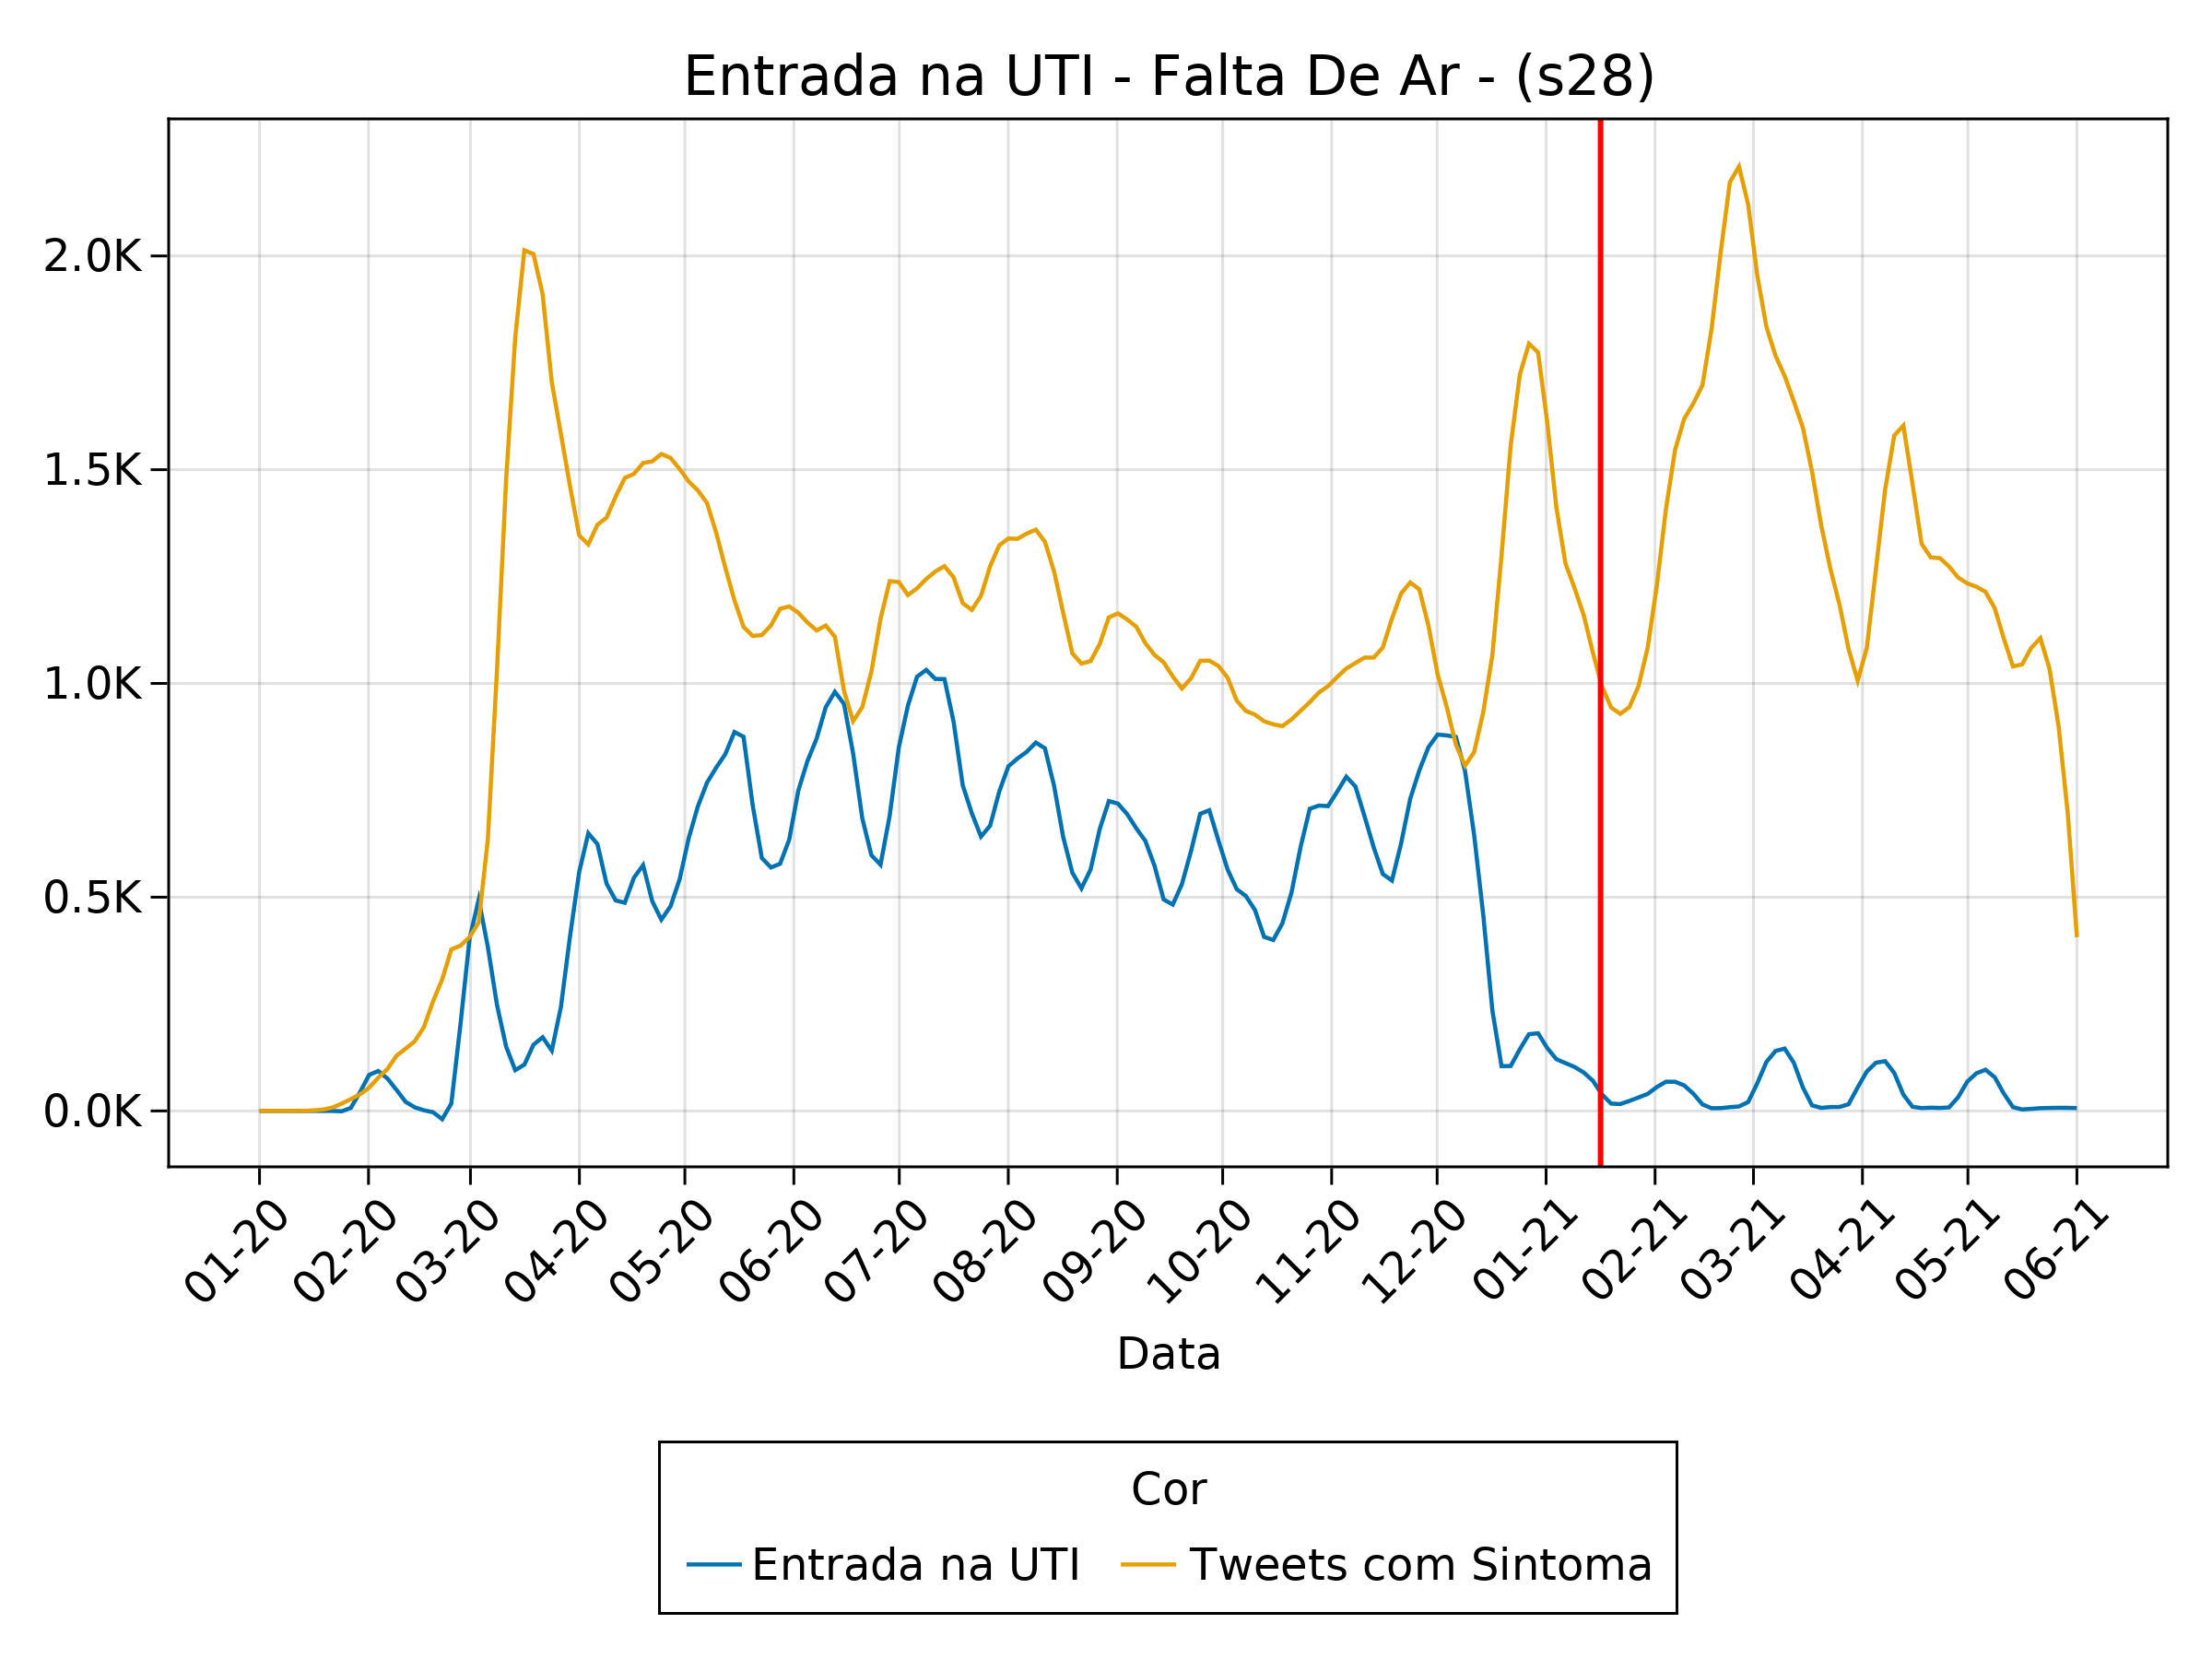
\includegraphics[width=0.6\textwidth]{srag_twitter_s28_ent.png}
        \label{fig:srag_twitter_s28_ent}
    \end{figure}
\end{frame}

\begin{frame}{Prova de Conceito - Paper no arXiv \parencite{storopoliSimulationDrivenCOVID19Epidemiological2021a}}
    Com 9.600 tweets anotados, conseguimos acurácia de 90\% no conjunto de dados de teste (quebra de 80\%/20\%)
    \vfill
    \begin{table}
        \centering
        \begin{tabular}{|c | c c c|}
            \hline
            rótulo & precisão\footnote{também chamada de valor preditivo positivo} & sensibilidade\footnote{também conhecida como revocação ou \textit{recall}} & score F1 \\
            \hline
            0 & 0.94 & 0.93 & 0.93 \\
            1 & 0.75 & 0.80 & 0.78 \\
            \hline
        \end{tabular}
        \label{tab:result_arXiv_classifier}
        \caption{Resultados do Classificador de Sintomas de Tweets Brasileiros}
    \end{table}
\end{frame}

\begin{frame}{Prova de Conceito - Paper no arXiv \parencite{storopoliSimulationDrivenCOVID19Epidemiological2021a}}
    \begin{figure}
        \centering
        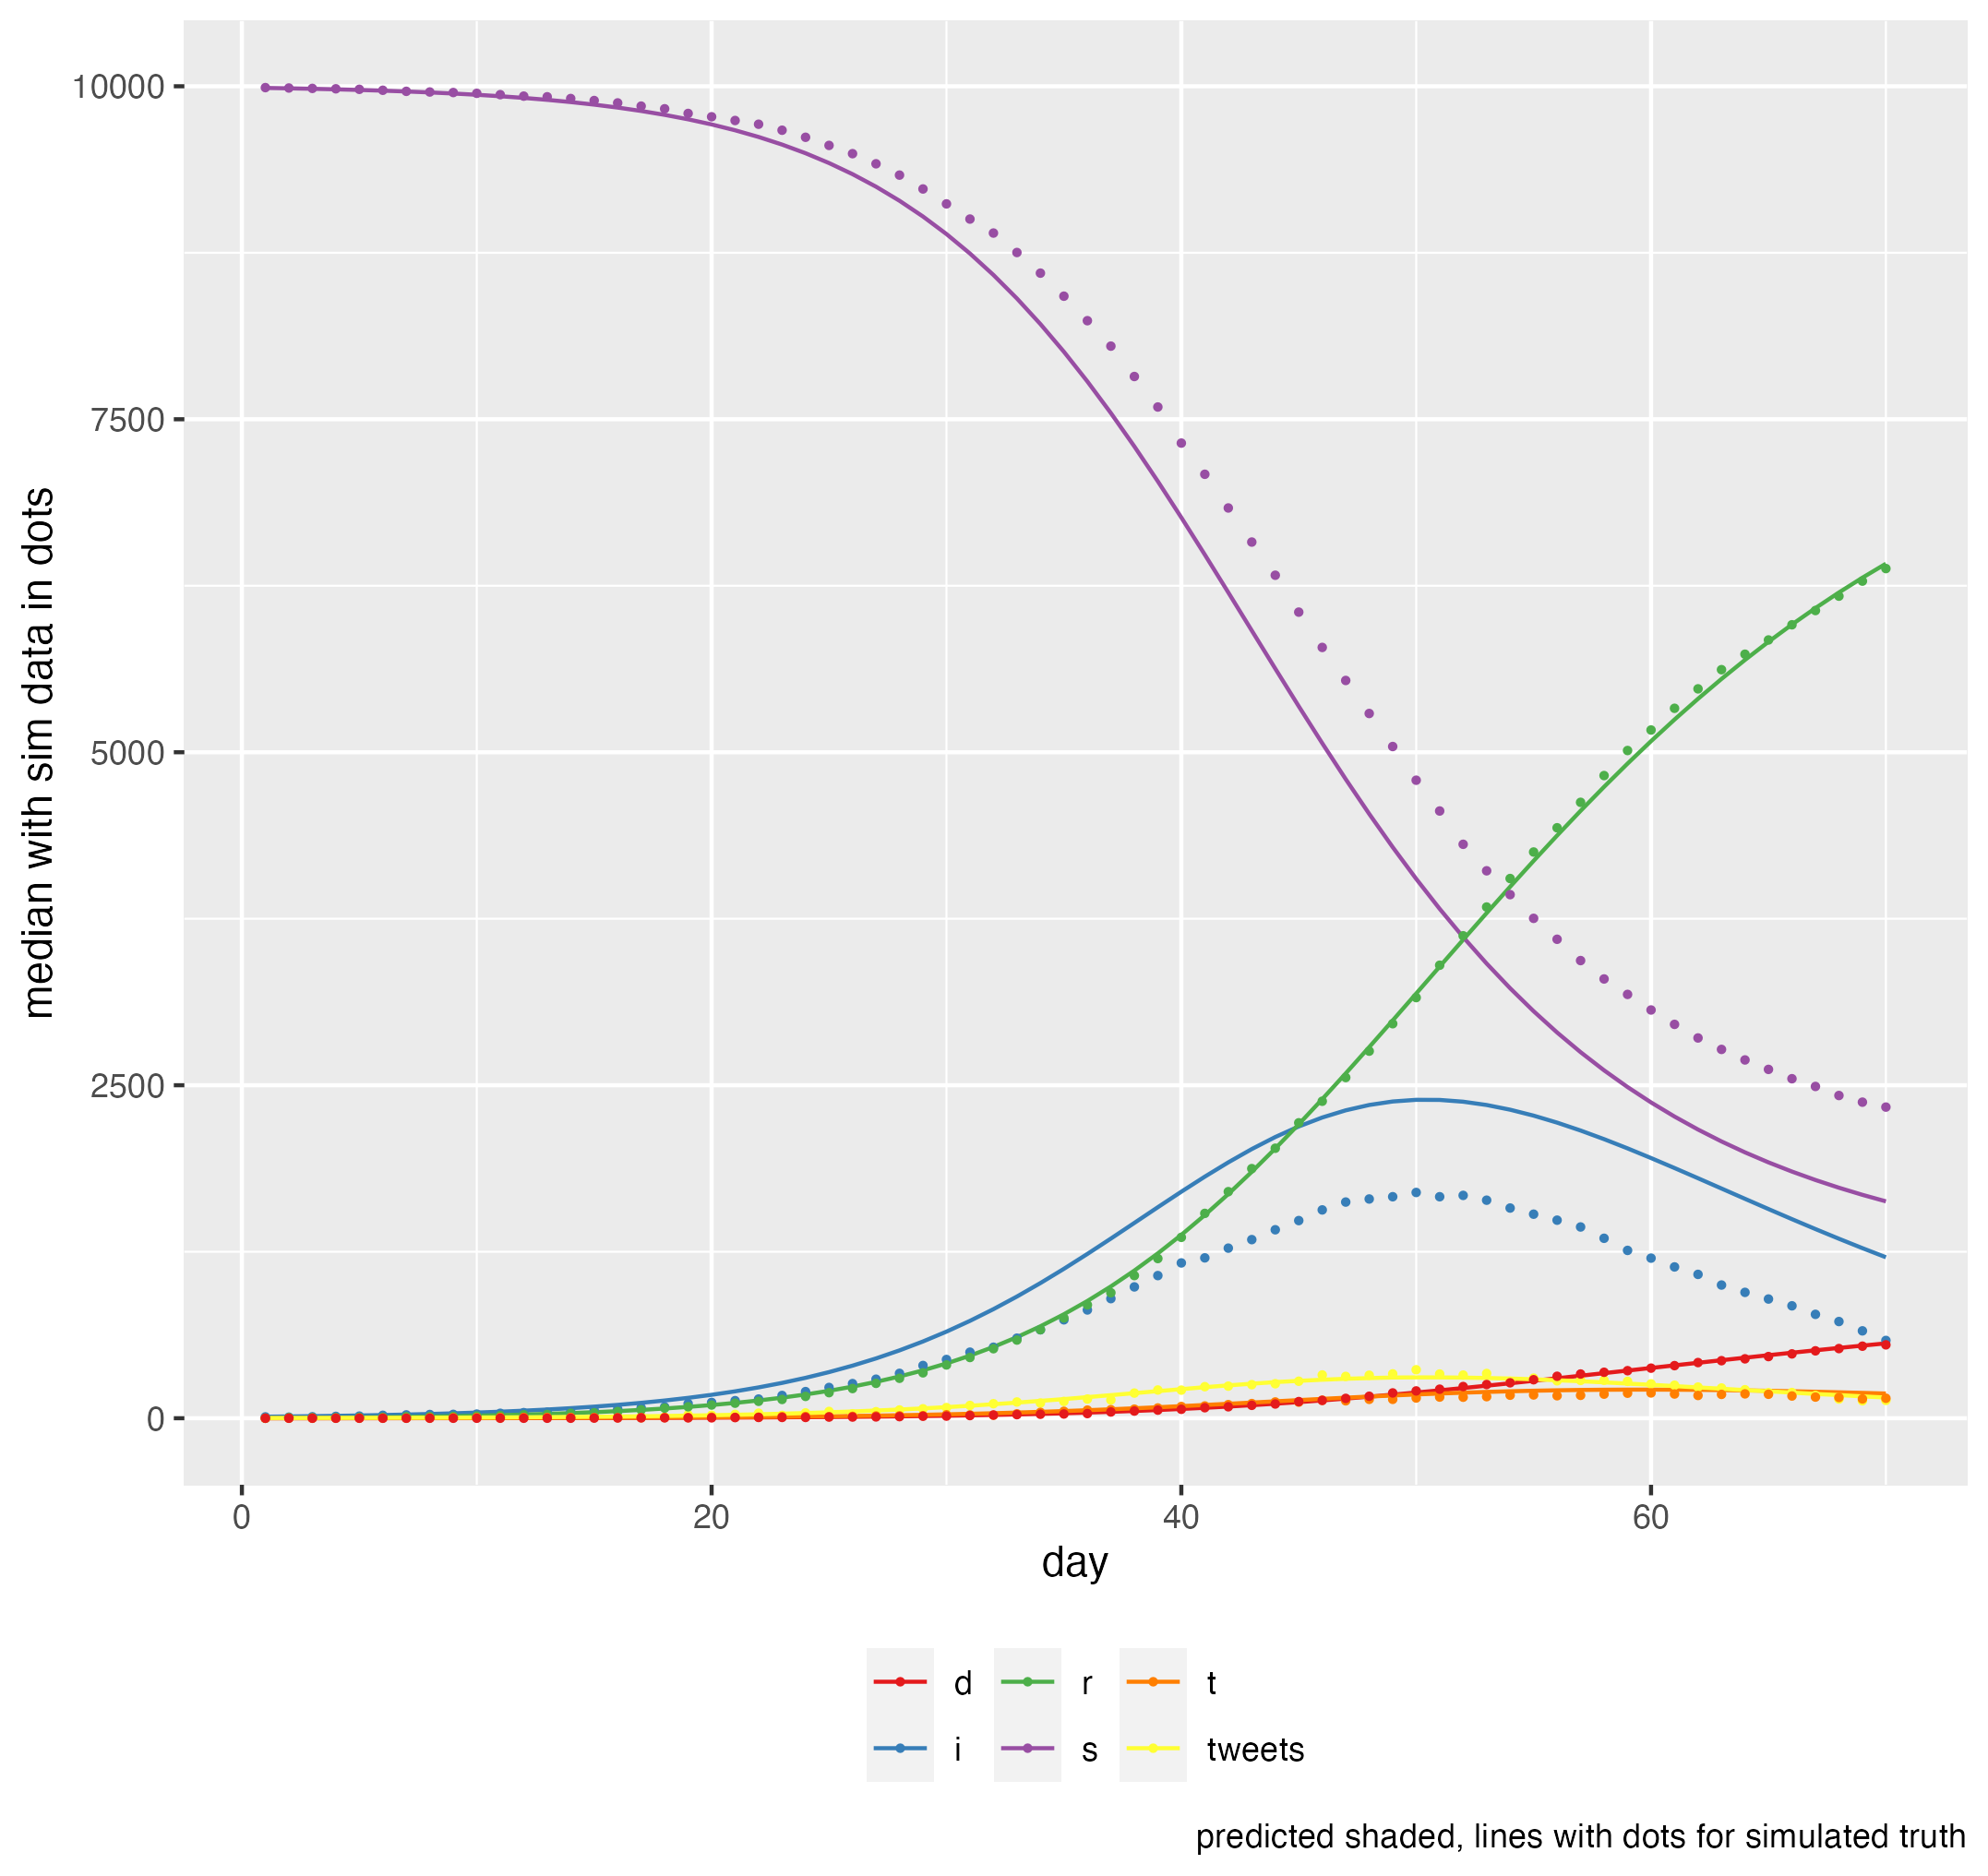
\includegraphics[width=0.45\textwidth]{fit_simulated.png}
        \caption{Dados Simulados versus Estimativas do Modelo}
        \label{fig:fit_simulated}
    \end{figure}
\end{frame}

\begin{frame}{Prova de Conceito - Paper no arXiv \parencite{storopoliSimulationDrivenCOVID19Epidemiological2021a}}
    \begin{figure}
        \centering
        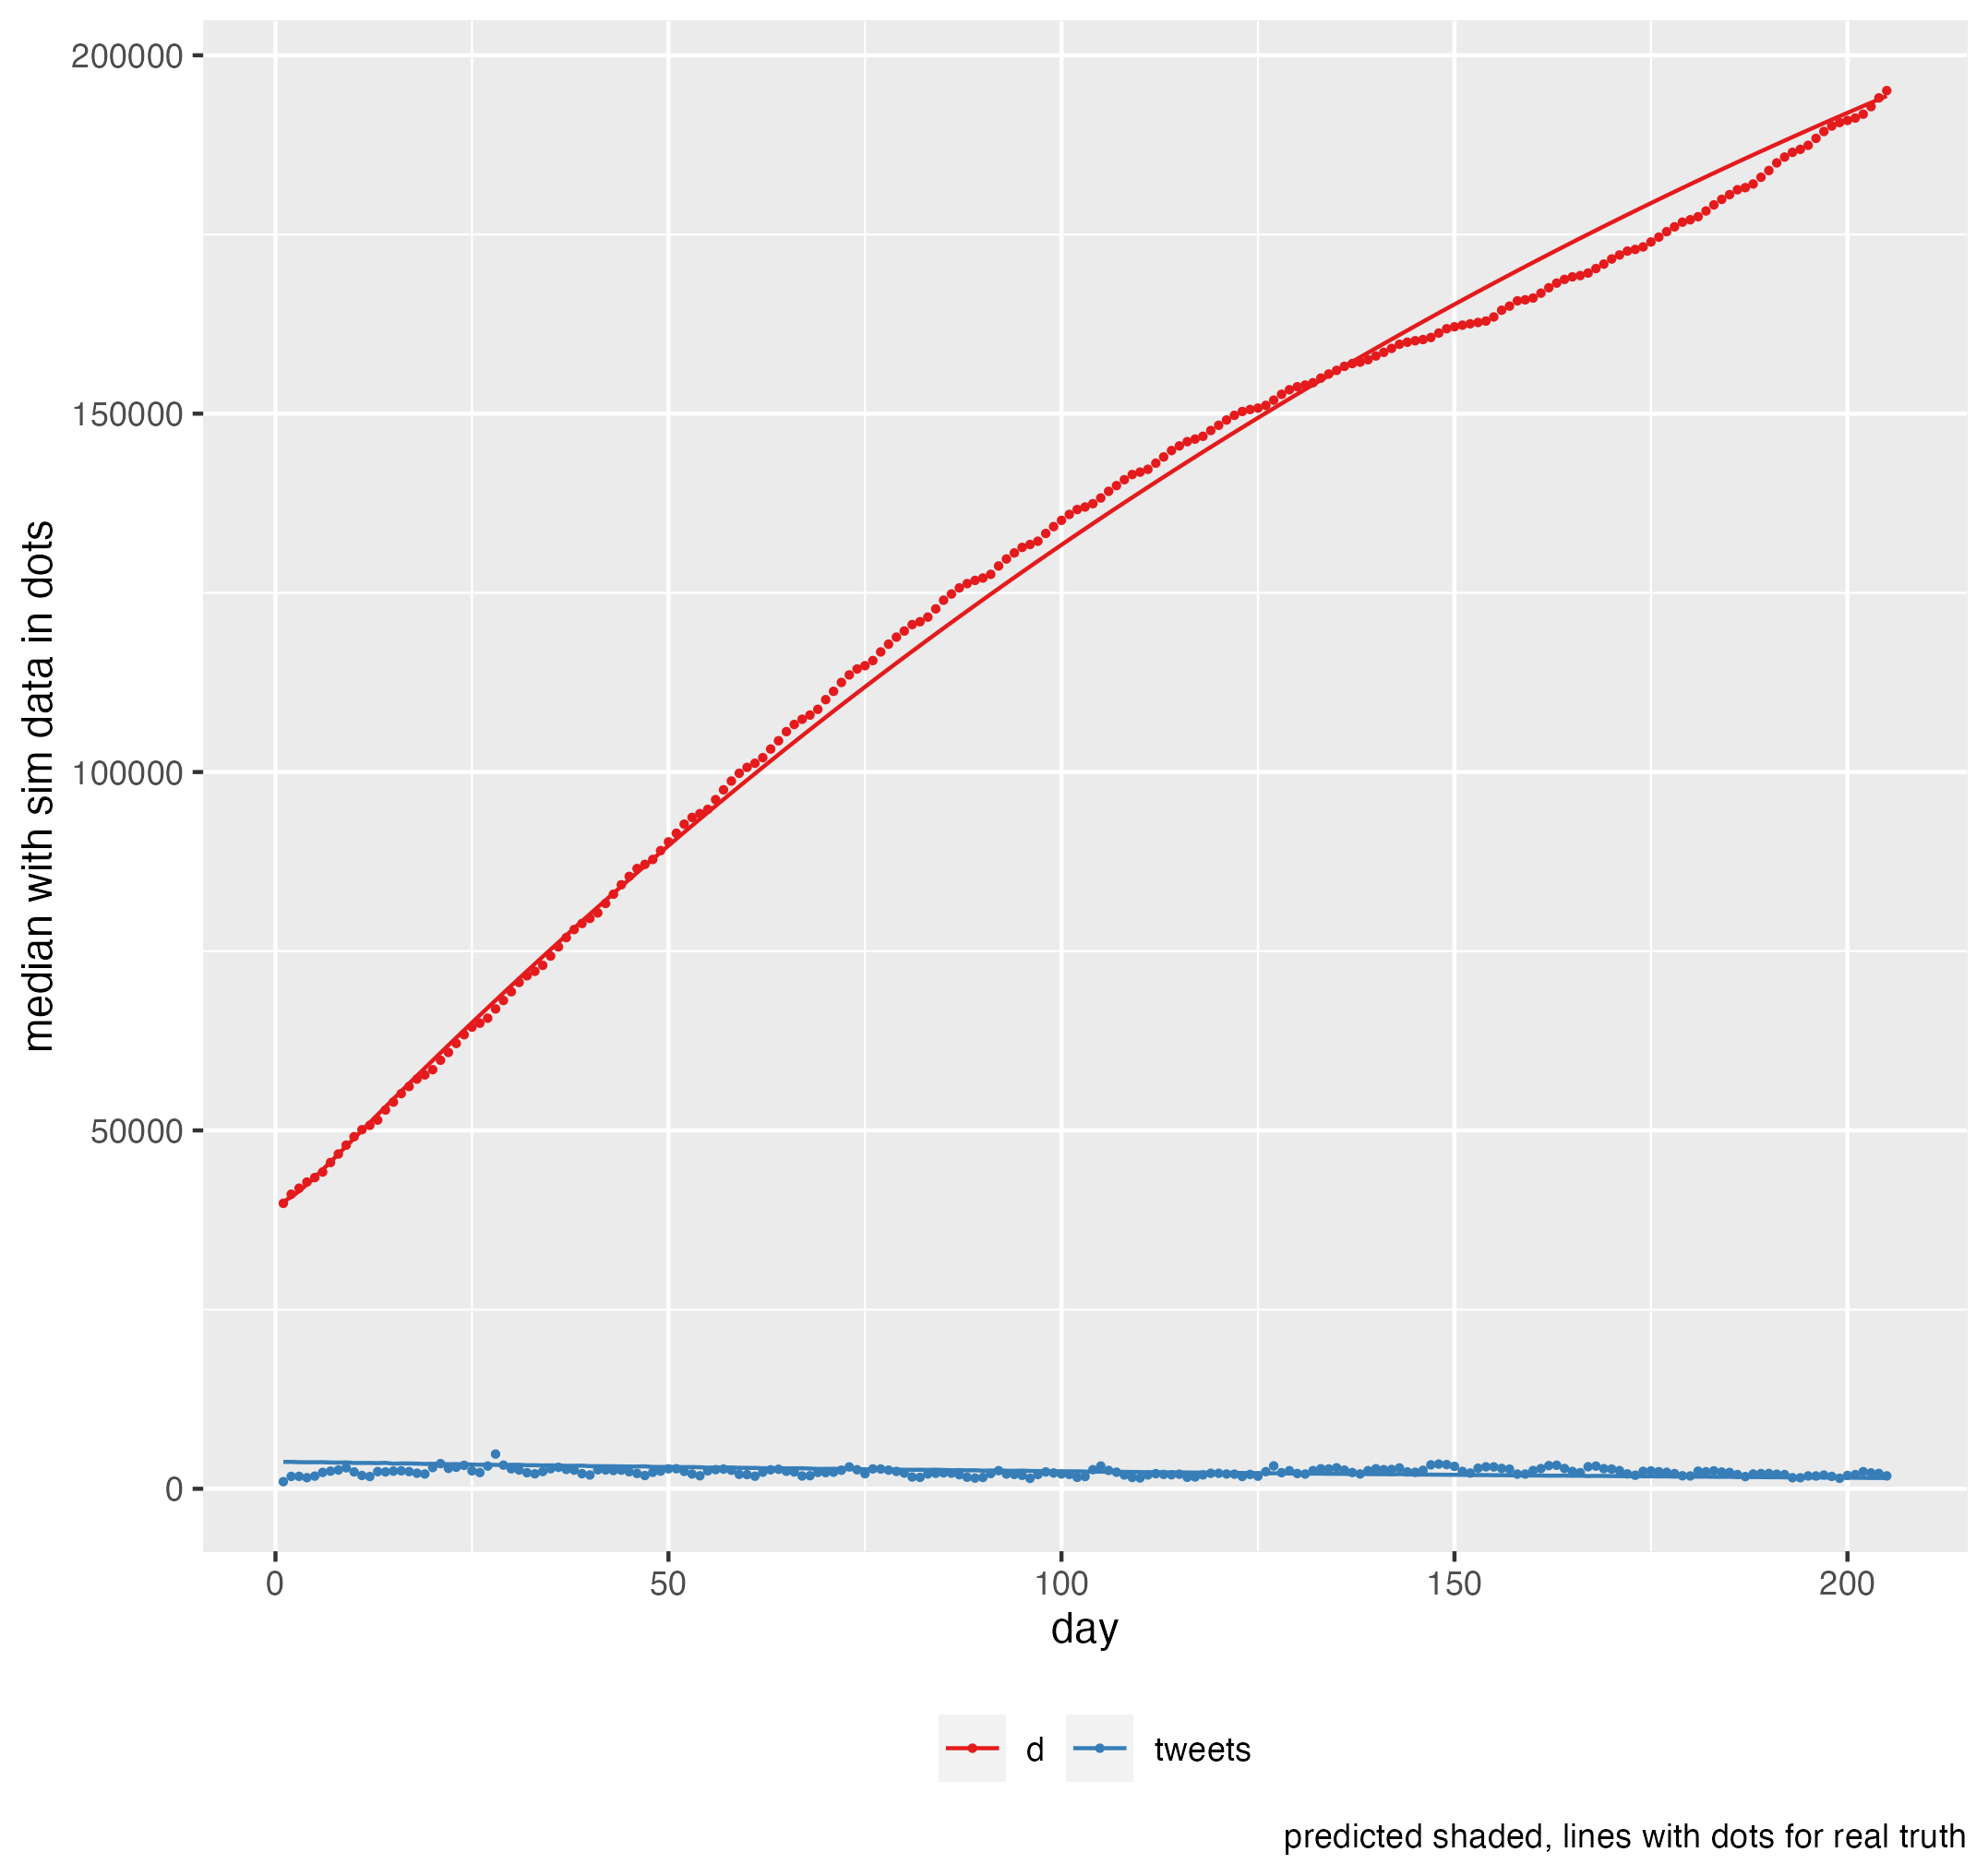
\includegraphics[width=0.45\textwidth]{fit_brazil.png}
        \caption{Dados do Brasil 2020 versus Estimativas do Modelo}
        \label{fig:fit_brazil}
    \end{figure}
\end{frame}

\section{Próximos Passos}
\begin{frame}{Próximos Passos - Classificador de Tweets}
    \begin{vfilleditems}
        \item Aprendizagem de máquina com diferentes modelos (Teorema do Almoço Grátis\footnote{\textit{No Free Lunch Theorem}} \parencite{wolpertLackPrioriDistinctions1996})
        \item Aprendizagem profunda com redes neurais e técnicas de Processamento de Linguagem Natural (PLN)
        como por exemplo o BERT\footnote{Bidirectional Encoder Representations from Transformers} \parencite{devlinBERTPretrainingDeep2018}
        já usado por \textcite{Kaushal_2020,santosh2020detecting} em redes sociais no contexto de COVID-19.
    \end{vfilleditems}
    %
    %
\end{frame}

\begin{frame}{Próximos Passos - Modelo Epidemiológico Bayesiano}
    \begin{vfilleditems}
        \item incorporar sintomas do Twitter
        \item taxa de contágio variável $\boldsymbol{\beta}$ (exemplo em \textcite{jaganFastEstimationTimevarying2020})
        \item tempo médio que os indivíduos estão em estado terminal variável $\boldsymbol{d_T}$
        \item inserção de vacinação (ver seção 4.3 de \textcite{gleesonCalibratingCOVID19SEIR2021})
        \item hierarquização do modelo para estados/regiões do Brasil (complicados pressupostos de estratificação de tweets)
    \end{vfilleditems}
\end{frame}

\begin{frame}{Próximos Passos - Rede Neural no Modelo Epidemiológico}
    Redes Neurais são aproximadores universais de funções \parencite{zubovNeuralPDEAutomatingPhysicsInformed2021}
    \begin{columns}
        \begin{column}{0.5\textwidth}
            \begin{vfilleditems}
                \item Rede neural para prever a relação não-linear e complexa entre $S$ e $I$ \parencite{pereiraDeepLearningBased2021}
                \item Rede neural para prever a relação entre $I$ e menções de sintomas
            \end{vfilleditems}
        \end{column}
        \begin{column}{0.6\textwidth}
            \begin{figure}
                \centering
                \begin{tikzpicture}[node distance=0.75cm,auto,>=latex',
                                    every node/.append style={align=center},
                                    state/.style={draw, circle, minimum size=0.9cm},
                                    neuralnetwork/.style={node contents=\usebox{\Chart}, minimum size=1.8cm}]
                    \node [state] (S) {$S$};
                    \begin{scope}[scale=0.75,
                                  nodes=neuralnetwork,
                                  every node/.append style={transform shape}]
                        \node(NN) [right= of S];
                    \end{scope}
                    % \pic [scale=0.1, right= of S] {neuralnetwork={2}{3}{1}};
                    \begin{scope}[node distance=0.5cm]
                        \node [state, right=of NN] (I) {$I$};
                    \end{scope}
                    \node [state, above right=of I] (T) {$T$};
                    \node [state, below right=of I] (R) {$R$};
                    \node [state, right=of T] (D) {$D$};

                    % \path[->, auto=false] (S) edge node {$\beta S \frac{I}{N}$ \\[2.5em]} (I);
                    \path[->, auto=false] (S) edge node {} (NN);
                    \path[->, auto=false] (NN) edge node {} (I);
                    \path[->, auto=false] (I) edge node {$\hspace{-1.75em} \frac{1}{d_I} I \omega$ \\[1.0em]} (T);
                    \path[->, auto=false] (I) edge node {$\hspace{5em} \frac{1}{d_I} I (1 - \omega)$ \\[1.2em]} (R);
                    \path[->, auto=false] (T) edge node {$\frac{1}{d_T} T$ \\[2.5em]} (D);
                \end{tikzpicture}
                \label{fig:SIRTD_neuralnetwork}
                \caption{Modelo SIRTD com Rede Neural}
            \end{figure}
        \end{column}
    \end{columns}
\end{frame}

\section{Referências}
\begin{frame}[allowframebreaks]{Referências}
    \printbibliography
\end{frame}

\appendix % do not count the following slides for the total number
\section*{Slides de Backup}
\begin{frame}[plain, noframenumbering]
    \centering
    \vfill
    {\fontsize{40}{50}\selectfont Backup Slides}
    \vfill
\end{frame}

\begin{frame}{Estatística Bayesiana}
    A estatística Bayesiana
    é uma abordagem de \textbf{análise de dados baseada no teorema de Bayes,
    onde o conhecimento disponível sobre os parâmetros em um modelo estatístico
    é atualizado com as informações dos dados observados}
    \parencite{gelman2013bayesian, mcelreath2020statistical}. O conhecimento prévio é expresso como
    uma distribuição
    \textit{a priori}
    e combinado com os dados observados na forma de uma função de
    verossimilhança
    para determinar a distribuição
    posterior.
    A posterior também pode ser usada para fazer previsões sobre eventos futuros.
\end{frame}

\begin{frame}{Inferência Bayesiana}
    $$
    \underbrace{P(\theta \mid y)}_{\text{Posterior}} = \frac{\overbrace{P(y \mid  \theta)}^{\text{Verossimilhança}} \cdot \overbrace{P(\theta)}^{\textit{Priori}}}{\underbrace{P(y)}_{\text{Constante Normalizadora}}}
    $$
    \begin{vfilleditems}
        \item \footnotesize $\theta$ -- parâmetro(s) de interesse
        \item \footnotesize $y$ -- dados observados
        \item \footnotesize \textbf{\textit{Priori}}: probabilidade prévia do valor do(s) parâmetro(s)
        \item \footnotesize \textbf{Verossimilhança}: probabilidade dos dados observados condicionados aos valores do(s) parâmetro(s)
        \item \footnotesize \textbf{Posterior}: probabilidade posterior do valor do(s) parâmetros após observamos os dados $y$
        \item \footnotesize \textbf{Constante Normalizadora}: $P(y)$ não faz sentido intuitivo. Essa probabilidade é transformada e pode ser interepretada como algo que existe apenas para que o resultado de $P(y \mid \theta) P(\theta)$ seja algo entre 0 e 1 -- uma probabilidade válida.
    \end{vfilleditems}
\end{frame}

\begin{frame}{Teorema de Bayes como Motor de Inferência}
    A estatísica Bayesiana nos permite \textbf{quantificar diretamente a incerteza}
    relacionada ao valor de um ou mais parâmetros do nosso modelo condicionado aos
    dados observados. Isso é a \textbf{característica principal} da estatística
    Bayesiana. Pois estamos estimando diretamente $P(\theta \mid y)$ por meio do
    teorema de Bayes. A estimativa resultante é totalmente intuitiva:
    simplesmente quantifica a intercerteza que temos sobre o valor de um ou mais
    parâmetro condicionado nos dados, nos pressupostos do nosso modelo
    (verossimilhança) e na probabilidade prévia que temos sobre tais valores.
\end{frame}

\begin{frame}{O que muda da Estatística Frequentista?}
    \begin{vfilleditems}
        \item \textbf{Flexibilidade} - peças probabilísticas para construir um modelo\footnote{como se fosse LEGO}:
            \begin{vfilleditems}
                \item Conjecturas probabilísticas sobre os parâmetros:
                \begin{vfilleditems}
                    \item \textit{Priori}
                    \item Verossimilhança
                \end{vfilleditems}
            \end{vfilleditems}
        \item Melhor tratamento da \textbf{incerteza}:
        \begin{vfilleditems}
            \item Coerência
            \item Propagação
            \item Não se usa \textit{"se amostrássemos infinitamente de uma população que não existe..."}
        \end{vfilleditems}
        \item Sem \textbf{$p$-valores}:
        \begin{vfilleditems}
            \item Todas as intuições estatísticas fazem \textbf{sentido}
            \item 95\% de certeza que o valor do parâmetro $\theta$ está entre $x$ e $y$
            \item Quase \textbf{impossível} fazer $p$-hacking.
        \end{vfilleditems}
\end{vfilleditems}
\end{frame}

\begin{frame}{Estatística Bayesiana vs Frequentista}
    \begin{table}[h!]
        \small
        \begin{tabular}{|l|p{.3\textwidth}|p{.3\textwidth}|}
        \toprule
                                & \textcolor{blue}{\textbf{Estatística Bayesiana}} & \textcolor{red}{\textbf{Estatística Frequentista}}                   \\ \midrule
        \textbf{Dados}          & Fixos –- Não Aleatórios                          & Incertos –- Aleatórios                                               \\ \midrule
        \textbf{Parâmetros}     & Incertos –- Aleatórios                           & Fixos –- Não Aleatórios                                              \\ \midrule
        \textbf{Inferência}     & Incerteza sobre o valor do parâmetro             & Incerteza sobre um processo de amostragem de uma população infinita  \\ \midrule
        \textbf{Probabilidade}  & Subjetiva                                        & Objetiva (mas com diversos pressupostos dos modelos)                 \\ \midrule
        \textbf{Incerteza}      & Intervalo de Credibilidade –- $P(\theta \mid y)$ & Intervalo de Confiança –- $P(y \mid \theta)$                         \\
        \bottomrule
        \end{tabular}
    \end{table}
\end{frame}

\begin{frame}{Vantagens da Estatística Bayesiana}
    \begin{vfilleditems}
        \item Abordagem Natural para expressar Incerteza
        \item Habilidade de incorporar Informações Prévias
        \item Maior Flexibilidade do Modelo
        \item Distribuição Posterior completa dos Parâmetros
        \item Propagação Natural da Incerteza
    \end{vfilleditems}
    \small \textbf{Principal Desvantagem}: Velocidade lenta de estimativa de modelos\footnote{\textit{e.g.} 30 segundos ao invés de 3 segundos na abordagem frequentista}
\end{frame}

\end{document}
